\documentclass[handout]{beamer}
\usepackage{verbatim}
\usepackage{xcolor}
\usepackage{multirow}
\usepackage{amssymb}
\usepackage{tikz}
\usetikzlibrary{positioning,fit}
%\usepackage{enumitem}
\usetheme{Warsaw}
\setbeamertemplate{navigation symbols}{}
\newcommand{\blue}[1]{{\color{blue} #1}}
\newcommand{\red}[1]{{\color{red} #1}}
\newcommand{\grn}[1]{{\color{green} #1}}
\newcommand{\bluRed}[2]{{\color{blue} #1}{\color{red} #2}}
\newcommand{\qtns}[0]{\begin{center} Questions? \end{center}}
\newcommand{\nl}[1]{\vspace{#1 em}}
\newcommand{\cntrImg}[2]{\begin{center}\includegraphics[scale=#2]{#1}\end{center}}
\newcommand{\defn}[1]{{\bf #1}}
\let\emptyset\varnothing
\newcommand{\SampS}[0]{$\mathcal{S}$}

\title{Math 3070, Applied Statistics}

\begin{document}

\begin{frame}
    \begin{beamercolorbox}[rounded=true,wd=\textwidth,center]{title}
        \usebeamerfont{title}\inserttitle
    \end{beamercolorbox}
    \begin{center}
        Section 1\\
        \nl{0.5}
        September 4, 2019
    \end{center}

\end{frame}

\begin{frame}{Lecture Outline, 9/4}
    Section 3.1
    \begin{itemize}
        \item Random Variables
        \item Probability Mass Functions
        \item Cumulative Distribution Function
        \item Examples
    \end{itemize}
\end{frame}

\begin{frame}{Random Variables}
    \begin{block}{defintion}
    A \textbf{random variable} is any rule that associates a number with each outcome in of a sample space, $\mathcal{S}$.
    \end{block}
    \begin{block}{notation}
        Most of the time random variables will be denoted with as capital case letters, $X,Y,Z,U,V$.\\
        \nl{0.5}
        When statement such as  $P(X=1)$ are writen this means the probability that the event $X=1$ occurs. To find the probability, one could find the probability of the event which yields $X=1$.
    \end{block}
    \begin{block}{foreshadowing}
        Later we will discuss random variables without explictly referring to an associated sample space, $\mathcal{S}$. The sample space is the outcomes of the random variable.
    \end{block}
\end{frame}

\begin{frame}{Random Variables, Discrete Versus Continuous}
    \begin{block}{discrete random variables}
        Random variables are \textbf{discrete} if they can take finitely many or countably many values. \textbf{Countably many} means the values can be listed one by one. For example, the integers and whole numbers are countable.
    \end{block}
    \begin{block}{continuous random variables}
        A random variables is \textbf{continuous} when
        \begin{enumerate}
            \item its possible values contain on any interval
            \item and the probability that it take on exactly one value is one, $P(X=c) = 0$ for all $c$.
        \end{enumerate}
        Random variables which take values on anywhere on the number line, an interval or half line, and satisfy property 2 are continuous random variables.
    \end{block}
\end{frame}

\begin{frame}{Discrete Random Variable Example, Die Roll}
    Example: Suppose we roll one fair six-sided die. The outcome of the roll is event that it lands on $1,2,3,4,5$ or $6$. Naturally, the number associated with the outcome is a random variable. 
    \end{frame}

\begin{frame}{Discrete Random Variable Example, Coin Flips}
Example: Suppose we toss a fair coin 3 times. The set of outcomes is
$$\Omega=\{(TTT),(TTH),(THT),(THH),(HTT),(HTH),(HHT),(HHH)\}$$
Let $X$ be the number of heads. Then $X$ is a random variable:
\begin{center}\begin{tabular}{p{4cm}p{4cm}}
\begin{tabular}{l}
$\begin{aligned}
TTT: X&=0 \\
TTH: X&=1 \\
THT: X&=1 \\
THH: X&=2
\end{aligned}$
\end{tabular} &
\begin{tabular}{l}
$\begin{aligned}
HTT: X&=1 \\
HTH: X&=2 \\
HHT: X&=2 \\
HHH: X&=3
\end{aligned}$
\end{tabular}
\end{tabular}
\end{center}
The possible values of $X$ are 0, 1, 2, and 3.\\
$X$ is a discrete random variable.
\end{frame}

\begin{frame}{Random Variables, Summary}
    \begin{itemize}
        \item Random variables are function that associate numbers to outcomes.
        \item Know the difference between discrete and continuous random variables. They will require different calculations.
        \item Mathematical expressions such as $P(X=5)$ and $P(X<3)$ read as the probability that the random variable $X$ takes the value $5$ or that probability that the random variable $X$ takes a value less than $3$. These are still probabilities of \underline{events}. This is why the previous rules of probability still apply.
    \end{itemize}
    \qtns
\end{frame}

\begin{frame}{Probability Mass Function, Definition}
    \begin{block}{defintion}
        The \textbf{probability mass function} (PMF) of a \underline{discrete} random variable is $f(x) = P(X = x)$.\\ \nl{0.5}
        $f(x)$ is a function.\\ \nl{0.5}
        $x$ is a varible, meaning that one may set it equal to numbers. \\ \nl{0.5}
        $P(X=x)$ is the probability that the event $X=x$ occurs.\\ \nl{0.5}
        PMFs only pertain to discrete random variables.
    \end{block}
\end{frame}

\begin{frame}{Probability Mass Function, Coin Flip Example}
    Consider the flip of a fair coin. The random variable $X$ takes $1$ if the coin lands on heads and $0$ if the coin lands on tails. Find the probability mass function of $X$.

    \pause
    $$
    f(x)= \left\{\begin{array}{lr}
        \frac{1}{2}, &  x = 0\\
        \frac{1}{2}, & x = 1\\
        0, & \text{otherwise}\\
        \end{array}\right.$$

        \pause
\begin{block}{definition}
    A \textbf{Bernoulli} random variable is one which only takes $0$ or $1$ as values. Note, the probabilities do not need to be 1/2.
\end{block}

    \end{frame}

\begin{frame}{Probability Mass Function, Die Roll Example}
    Consider $X$ the value yielded from a single roll of a fair six-sided die. Determine the probabilty mass function.

    \pause There is a 1/6 probabilty of observing any side.
    $$
    f(x)= \left\{\begin{array}{lr}
        \frac{1}{6}, & x = 1,2,3,4,5,6\\
        0, & \text{otherwise}\\
        \end{array}\right.$$
\hfill
    \end{frame}

\begin{frame}{Probability Mass Function, Coin Flips Example}
    In the previous example, we can calculate the probability of the number of heads out of 3 coins flips $X$ being each of the values 0, 1, 2, and 3:
    \begin{align*}
    &P(X=0) = P(\{TTT\}) = 1/8 \\
    &P(X=1) = P(\{HTT, THT, TTH \}) = 3/8 \\
    &P(X=2) = P(\{HHT, HTH, THH\}) = 3/8 \\
    &P(X=3) = P(\{HHH\}) = 1/8
    \end{align*}
    \pause The PMF, $f(x)=P(X=x)$, describes the probability of each possible value:
    \begin{center}
    \begin{tabular}{p{6cm}p{6cm}}
    \vspace{-1cm}
    $$
    f(x)= \left\{\begin{array}{lr}
        1/8, & \text{for } x = 0\\
        3/8, & \text{for } x = 1\\
        3/8, & \text{for } x = 2\\
        1/8, & \text{for } x = 3\\
        0, & \text{otherwise}\\
        \end{array}\right.$$&
    \vspace{-2cm}
    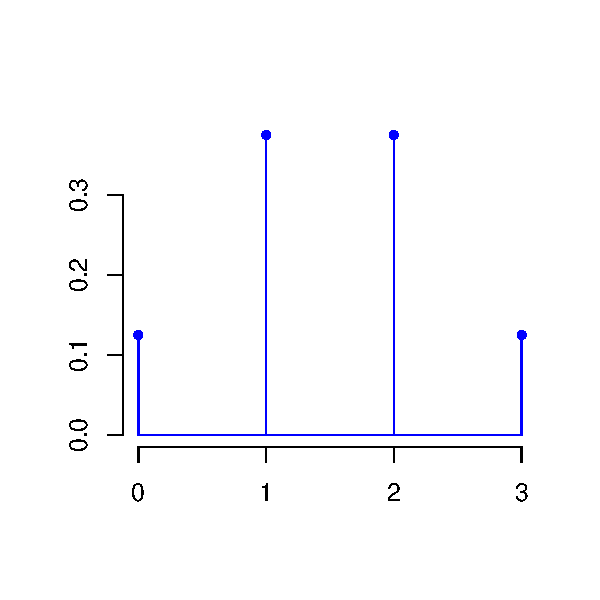
\includegraphics[scale=.5]{ch3_pmf.pdf}
    \end{tabular}
    \end{center}
\end{frame}

\begin{frame}{Sum of Two Random Variables}
    Suppose we roll two six-sided dice, and let $X$ and $Y$ be the results. Their sum is a random variable $X+Y$ with values 2, 3, \dots, 12. What is the probability mass function of $X+Y$?
    
    \pause\vspace{-.5cm}\begin{center}
    \begin{tabular}{p{4.7cm}p{5.5cm}}
    \vspace{0cm}
    \begin{tabular}{l||p{.3cm}|p{.3cm}|p{.3cm}|p{.3cm}|p{.3cm}|p{.3cm}|}
    & 1 & 2 & 3 & 4 & 5 & 6 \\ \hline \hline
    1& 2 & 3 & 4 & 5 & 6 & 7 \\ \hline
    2& 3 & 4 & 5 & 6 & 7 &  8  \\ \hline
    3& 4 & 5 & 6 & 7 &  8 & 9 \\ \hline
    4& 5 & 6 & 7 &  8 & 9 & 10\\ \hline
    5& 6 & 7 &  8 & 9 &10 & 11\\ \hline
    6& 7 &  8 & 9 & 10 & 11 & 12\\ \hline
    \end{tabular}
    &
    \vspace{-1.5cm}
    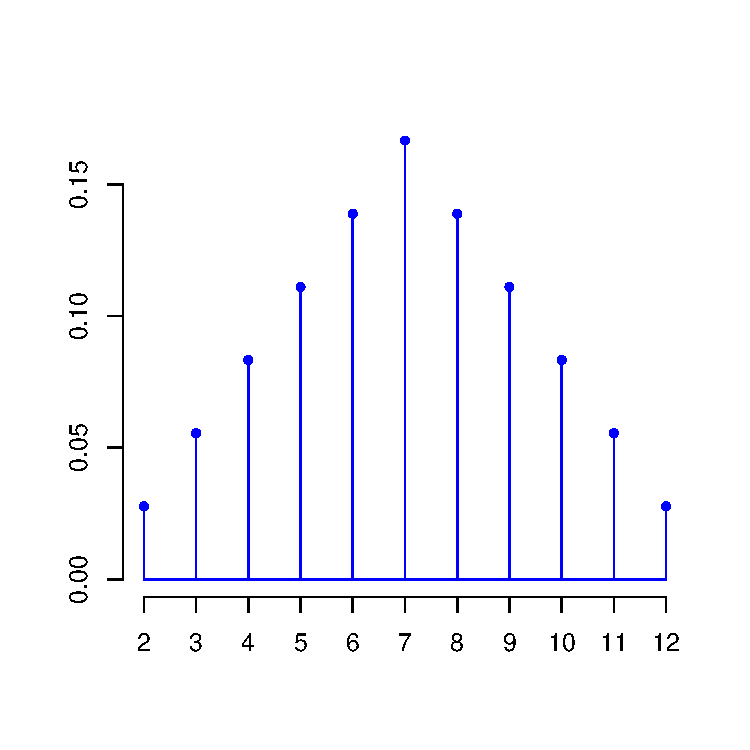
\includegraphics[scale=.5]{ch3_pmf2.pdf}
    \end{tabular}
    
    \vspace{-.5cm}
    \renewcommand{\arraystretch}{1.5}
    \begin{tabular}{c||c|c|c|c|c|c|c|c|c|c|c|}
    $x$ & 2 & 3 & 4 & 5 & 6 & 7 & 8 & 9 & 10 & 11 & 12 \\ \hline
    $f(x)$ & $\frac1{36}$ & $\frac2{36}$ & $\frac3{36}$ & $\frac4{36}$ & $\frac5{36}$ & $\frac6{36}$ & $\frac5{36}$ & $\frac4{36}$ & $\frac3{36}$ & $\frac2{36}$ & $\frac1{36}$
    \end{tabular}
    \end{center}
\end{frame}

\begin{frame}{Sum of Two Random Variables}
    Suppose we roll two six-sided dice, and let $X$ and $Y$ be the results. Their sum is a random variable $X+Y$ with values 2, 3, \dots, 12. What is the probability that $X+Y$ is even?  What is the probability that $X+Y$ is less than 5.
    
    \begin{center}
    \renewcommand{\arraystretch}{1.5}
    \begin{tabular}{c||c|c|c|c|c|c|c|c|c|c|c|}
    $x$ & 2 & 3 & 4 & 5 & 6 & 7 & 8 & 9 & 10 & 11 & 12 \\ \hline
    $f(x)$ & $\blue{\frac1{36}}$ & $\frac2{36}$ & $\blue{\frac3{36}}$ & $\frac4{36}$ & $\blue{\frac5{36}}$ & $\frac6{36}$ & $\blue{\frac5{36}}$ & $\frac4{36}$ & $\blue{\frac3{36}}$ & $\frac2{36}$ & $\blue{\frac1{36}}$
    \end{tabular}
    \end{center}
    \pause
    $$P("X+Y \text{ is even}") = \frac1{36} + \frac3{36} + \frac5{36} + \frac5{36} + \frac3{36} + \frac1{36} = \frac{18}{36}$$
\end{frame}

\begin{frame}{Sum of Two Random Variables}
    Suppose we roll two six-sided dice, and let $X$ and $Y$ be the results. Their sum is a random variable $X+Y$ with values 2, 3, \dots, 12. What is the probability that $X+Y$ is less than 6?
    
    \begin{center}
    \pause \begin{tabular}{c||c|c|c|c|c|c|c|c|c|c|c|}
    $x$ & 2 & 3 & 4 & 5 & 6 & 7 & 8 & 9 & 10 & 11 & 12 \\ \hline
    $f(x)$ & $ \red{\frac1{36}}$ & $\red{\frac2{36}}$ & $\red{\frac3{36}}$ & $\red{\frac4{36}}$ & $\frac5{36}$ & $\frac6{36}$ & $\frac5{36}$ & $\frac4{36}$ & $\frac3{36}$ & $\frac2{36}$ & $\frac1{36}$
\end{tabular}
\end{center}
    \pause
    $$ P(X+Y<6) = \frac{1}{36} + \frac{2}{36} + \frac{3}{36} + \frac{4}{36} = \frac{10}{36}$$
    Note:
    $$ P(X+Y < 6) = P(X+Y \leq 5) $$
    
\end{frame}

\begin{frame}{Probability Mass Function, Summary and Comments}
    \begin{itemize}
        \item The Probability Mass Function $f(x)$ is a function whose input are numbers $x$ and whose output is the probability of its associate discrete random variable $X$ taking that number.
        \item Only relevant for discrete random variables.
        \item A Bernoulli random variable is one which only takes $0$ or $1$ as values.
        \item Take care to distingush $<$ and $\leq$ in events.
        \item The sum of the PMF over all possible values of the random variable must be 1, $P(\mathcal{S})=1$.
        \item If the PMF is known, the behavior of the discrete random varible is known.
    \end{itemize}
\end{frame}

\begin{frame}{Cumulative Distribution Function, Definition}
    \begin{block}{definition}
    The \textbf{cumulative distribution function} (CDF) $F(x)$ of a discrete random variable $X$ with PMF $f(x)$ is defined for every number $x$ by
    $$F(x) = P(X \leq x) = \sum_{y:y\leq x} p(y).$$
    \end{block}
    $F(x)$ is also the probability that $X$ is at most $x$. \\ \nl{0.5}
    Compute $F(x)$ by computing the running total. 
\end{frame}

\begin{frame}{Cumulative Distribution Function, Coin Flips Example}
        Suppose flip 3 coins. Calculate the CDF of $X$ the number of heads out of 3 coin flips.
        
    $$
    f(x)= \left\{\begin{array}{lr}
        1/8, & \text{for } x = 0\\
        3/8, & \text{for } x = 1\\
        3/8, & \text{for } x = 2\\
        1/8, & \text{for } x = 3\\
        0, & \text{otherwise}\\
        \end{array}\right.$$
        \pause$$
    F(x)= \left\{\begin{array}{lr}
        0, & \text{for } x < 0\\
        \pause 1/8, & \text{for } 0 \leq x < 1\\
        \pause 4/8, & \text{for } 1 \leq x < 2\\
        \pause 7/8, & \text{for } 2 \leq x < 3\\
        \pause 1, & 3\leq x\\
        \end{array}\right.$$
    \end{frame}

    \begin{frame}{Cumulative Distribution Function, Summary}
        \begin{itemize}
            \item $F(x) = P(X \leq x) = \sum_{y:y\leq x} p(y)$
            \item Probability that $X$ is at least $x$, this includes $x$.
            \item For $x$ strictly less than any observable value of $X$, the CDF is zero.
            \item For $x$ strictly greater than any observable value of $X$, the CDF is one.
            \item The "jumps" include the left endpoints.
        \end{itemize}
    \end{frame}

    \begin{frame}{Examples, Random Digits}
        A password generator samples numerical passwords of length of at most 4, equally likely. Consider $X$ is the length of the password. Compute the PDF and CDF of $X$.\\ \nl{0.5}
        \pause
        Count the total number of outcomes. \pause Each digit can be repeated and order matters. \pause k-tuple formula applies. Add number of passwords at each length.
        \pause $$ \text{total number of passwords} = 10 + 10^2 + 10^3 + 10^4= 11110$$
        \pause $$f(x)= \left\{\begin{array}{lr}
            10/11110, & x = 1\\
            100/11110, &  x = 2\\
            1000/11110, &  x = 3\\
            10000/11110, &  x = 4\\
            0, & \text{otherwise}\\
            \end{array}\right.$$
    \end{frame}

    \begin{frame}{Examples, Random Digits}
        A password generator samples numerical passwords of length at most 4, equally likely. Consider $X$ is the length of the password. Compute the PDF and CDF of $X$.\\ \nl{0.5}
        $$f(x)= \left\{\begin{array}{lr}
            10/11110, & x = 1\\
            100/11110, &  x = 2\\
            1000/11110, &  x = 3\\
            10000/11110, &  x = 4\\
            0, & \text{otherwise}\\
            \end{array}\right.$$
        \pause $$F(x)= \left\{\begin{array}{lr}
            0, & x<1\\
            10/11110, & 1 \leq x < 2\\
            110/11110, &  2 \leq x < 3\\
            1110/11110, &  3 \leq x < 2\\
            1, &  4 \leq x\\
            \end{array}\right.$$
    \end{frame}
    \begin{frame}{Examples, Nonexample}
        Is $f(x)$ a PMF?
        $$f(x)= \left\{\begin{array}{lr}
            \dfrac{x!}{3!}, & x = 0,1,2,3\\
            0, & \text{otherwise}\\
            \end{array}\right.$$
            \pause nope, $f(3)=1$ so we expect the sum over observable values to be greater than 1.
            \begin{align*}
                \sum_{x=0}^3 f(x) & = \frac{0!}{3!} + \frac{1!}{3!} +\frac{2!}{3!} +\frac{3!}{3!}\\
                 &= \frac{1}{6} + \frac{1}{6} +\frac{2}{6} +\frac{6}{6} \\
                 & = \frac{10}{6} = \frac{5}{3}
            \end{align*}

    \end{frame}
    \begin{frame}{Examples, Nonexample}
        Determine what value of $k$ ensures that $f(x)$ is a PMF?
        $$f(x)= \left\{\begin{array}{lr}
            k \dfrac{x!}{3!}, & x = 0,1,2,3\\
            0, & \text{otherwise}\\
            \end{array}\right.$$
            \pause $$k = \frac{3}{5}$$. We need the sum over all observable values to be $1$.
            $$ \sum_{x=0}^3 f(x)  = k \frac{0!}{3!} + k \frac{1!}{3!} + k\frac{2!}{3!} +k \frac{3!}{3!} = k \frac{5}{3} = 1$$
            
    \end{frame}

    \begin{frame}{Relation to Previous "Distributions"}
        The Probability Mass Function is also called the \textbf{probability distribution}. Recall that the distribution of data describes how frequently outcomes or value are observed and a frequentist model describes relative frequency. When we try to model experimental outcomes with  a random variable, comparing the PMF to the histogram helps judge the validity of the the probabilistic model. 
        \\ \nl{0.5}
        Moreover, modeling the connections between random variables extends probabilistic models into new settings. For example, you may not want the random variable itself, but a sum or product of them. We have already encountered a weight sum of random variables, the sample mean and variance.
        \begin{center}
            More on that in the next lecture\ldots
        \end{center}
    \end{frame}
\end{document}